\chapter{Architectures}

\textcolor{red}{Mention the different architectures, figures of their components, hyperparameters we tune on them, and motivation.}

\section{Recurrent Neural Network}

The \gls{RNN} is a standard architecture when it comes prediction on temporal data. It has been tried and tested, showing promising results for audio tasks.

The fundamental building block for \gls{RNN}s is the \textit{recurrent unit}. It stores information from previous timesteps in a form of memory, through maintenance of a \textit{hidden state}.

However, traditional \gls{RNN}s suffer from the \textit{vanishing gradient problem}, making \textit{long range dependencies} harder to learn. Different architectures have been developed to try to overcome these issues, such as the \gls{GRU} by Cho et al.~\cite{DBLP:conf/emnlp/ChoMGBBSB14}, and \gls{LSTM} by Hochreiter et al.~\cite{10.1162/neco.1997.9.8.1735}.

It has been shown that \gls{GRU}s and \gls{LSTM}s are capable of learning \gls{ADT} related tasks, and is therefore in interest to comparatively measure how their efficiency stands in regards to other architectures~\cite{Southall2016AutomaticDT, inproceedings, Vogl2017DrumTV, signals4040042}.

\subsection{Implementation}

Our \gls{RNN} architecture consists of several bilateral recurrent units, ending in a framewise linear layer. For the recurrent units, we train both a \gls{GRU} and an \gls{LSTM} model, in addition to hyperparameter search over $L \in \{2, 3, 4, 5, 6\}$ and $H \in \{72, 144, 288\}$, selecting the one with best performance.

\begin{figure}[H]
    \centering
    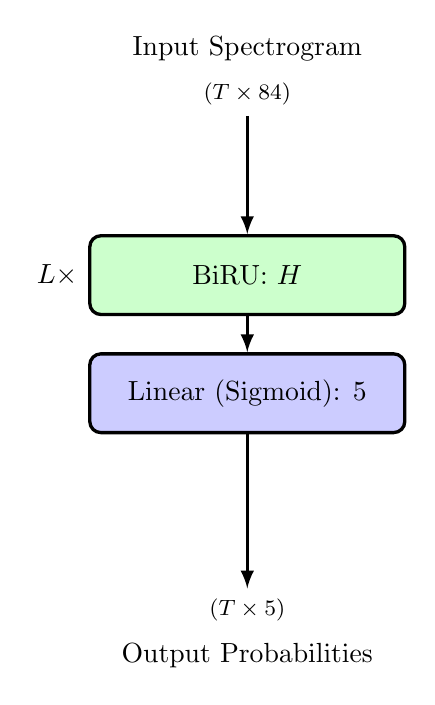
\begin{tikzpicture}[
    very thick,
    arrow/.style={
        -latex,
        very thick,
        rounded corners=0.2cm
    },
    ]

\node[anchor=south, label=above:{Input Spectrogram}] at (0, 0){\footnotesize{($T \times 84$)}};

\draw[arrow] (0, 0) -- (0, -1.5) node[rectangle, 
rounded corners, 
draw, 
anchor=north, 
label=west:$L\times$,
fill=green!20,
minimum height=1cm,
minimum width=4cm
] (a) {\acrshort{BiRU}: $H$};

\draw[arrow] (a) -- (0, -3) node[rectangle, 
rounded corners, 
draw, 
anchor=north, 
fill=blue!20,
minimum height=1cm,
minimum width=4cm
] (b) {Linear (Sigmoid): $5$};

\draw[arrow] (b) -- (0, -6);

\node[anchor=north, label=below:{Output Probabilities}] at (0, -6){\footnotesize{($T \times 5$)}};

\end{tikzpicture}
    \caption{RNN architecture structure.}
    \label{RNNFigure}
\end{figure}

\textcolor{red}{Show model architecture diagram like the one in ADTOF-YT paper}.

\section{Convolutional Neural Network}

\section{Convolutional Recurrent Neural Network}

\section{Convolutional Transformer}

\section{Vision Transformer}